% ============================================================
% BLG 632E — Next Generation Wireless Networks
% Term Project Presentation — Ömer Dikyol
% ============================================================
\documentclass[aspectratio=169,t]{beamer}

\usetheme{Madrid}
\usecolortheme{whale}

\usepackage[utf8]{inputenc}
\usepackage[T1]{fontenc}
\usepackage{amsmath,amssymb,amsfonts}
\usepackage{graphicx}
\usepackage{xcolor}
\usepackage{tikz}
\usetikzlibrary{arrows.meta,positioning,shapes.geometric,fit,backgrounds,calc,decorations.pathreplacing}
\usepackage{booktabs}
\usepackage{array}
\usepackage{textcomp}

\graphicspath{{../output/figures/}}

% ── Colours ─────────────────────────────────────────────────
\definecolor{ITUblue}{RGB}{0,60,130}
\definecolor{ITUred}{RGB}{190,30,45}
\definecolor{alertorange}{RGB}{220,100,0}
\definecolor{successgreen}{RGB}{0,130,60}
\definecolor{lightgray}{RGB}{240,240,245}
\colorlet{ITUblueMid}{ITUblue!50!white}
\colorlet{ITUblueLight}{ITUblue!25!white}

\setbeamercolor{structure}{fg=ITUblue}
\setbeamercolor{palette primary}{bg=ITUblue,fg=white}
\setbeamercolor{palette secondary}{bg=ITUblue!80,fg=white}
\setbeamercolor{palette tertiary}{bg=ITUblue!60,fg=white}
\setbeamercolor{palette quaternary}{bg=ITUblue,fg=white}
\setbeamercolor{alerted text}{fg=ITUred}
\setbeamercolor{block title alerted}{bg=ITUred!10,fg=ITUred}
\setbeamercolor{block body alerted}{bg=ITUred!5}
\setbeamercolor{block title example}{bg=successgreen!10,fg=successgreen!80!black}
\setbeamercolor{block body example}{bg=successgreen!5}
\setbeamertemplate{navigation symbols}{}

% ── Footer ──────────────────────────────────────────────────
\setbeamertemplate{footline}{%
  \leavevmode%
  \hbox{%
    \begin{beamercolorbox}[wd=\paperwidth,ht=2.25ex,dp=1ex,right]{date in head/foot}%
      \usebeamerfont{date in head/foot}\insertframenumber{} / \inserttotalframenumber\hspace{2em}%
    \end{beamercolorbox}}%
}

% ── Math macros ─────────────────────────────────────────────
\newcommand{\qreal}{Q_{\mathrm{real}}}
\newcommand{\qvirt}{Q_{\mathrm{virtual}}}
\newcommand{\pacb}{p_{\mathrm{acb}}}
\newcommand{\ema}{\mathrm{EMA}}

% ── TikZ styles ─────────────────────────────────────────────
\tikzset{
  box/.style={rectangle, rounded corners=4pt, draw=#1, fill=#1!12,
              minimum width=2.0cm, minimum height=0.85cm,
              font=\small\bfseries, text centered, align=center},
  arr/.style={-{Stealth[length=6pt]}, thick, #1},
  stage/.style={rectangle, rounded corners=5pt, draw=ITUblue, fill=ITUblue!10,
                minimum width=2.6cm, minimum height=1.0cm,
                font=\footnotesize\bfseries, text centered, align=center},
}

% =============================================================
\title[5G RRC Signaling Storm]{%
  5G RRC Signaling Storm Mitigation\\
  via a Proactive Digital Twin Architecture\\
  with Continuous Calibration}

\author[Omer Dikyol]{%
  \textbf{Omer Dikyol}\\[4pt]
  {\small Department of Computer Engineering}\\
  {\small Istanbul Technical University}}

\institute[ITU]{BLG 632E -- Next Generation Wireless Networks}

\date{Spring 2025--2026}

% =============================================================
\begin{document}
% =============================================================

% ── TITLE ────────────────────────────────────────────────────
{
\setbeamertemplate{footline}{}
\begin{frame}[noframenumbering]
  \titlepage
\end{frame}
}

% ── OUTLINE ──────────────────────────────────────────────────
\begin{frame}{Outline}
  \tableofcontents[hideallsubsections]
\end{frame}

% =============================================================
\section{Problem Definition \& Research Gap}
% =============================================================

% ── SLIDE: WHY 5G MATTERS ───────────────────────────────────
\begin{frame}{Motivation: Why 5G Availability Matters}

  \begin{columns}[T]
    \begin{column}{0.55\textwidth}
      \small
      \textbf{5G NR supports mission-critical services}

      \vspace{2pt}
      \begin{itemize}\setlength\itemsep{2pt}
        \item Autonomous vehicles require sub-10\,ms round-trip latency
        \item Remote surgery and industrial IoT need \textbf{five-nines reliability}
        \item Every device starts with an RRC connection request through the \textbf{gNB RACH}
      \end{itemize}

      \vspace{4pt}
      \textbf{Consequence of RACH failure}

      \vspace{2pt}
      \begin{itemize}\setlength\itemsep{2pt}
        \item No RACH access $\Rightarrow$ no data plane
        \item A single gNB serves hundreds to thousands of UEs simultaneously
        \item Overloading the RACH blocks \textbf{all} connected services
      \end{itemize}
    \end{column}

    \begin{column}{0.43\textwidth}
      \begin{block}{gNB RACH at a Glance}
        \small
        \begin{itemize}\setlength\itemsep{4pt}
          \item $c = 54$ preamble channels
          \item Buffer capacity $K = 200$
          \item Requests arriving when $\qreal \geq K$ are dropped immediately
        \end{itemize}
      \end{block}

      \vspace{10pt}
      \begin{alertblock}{Security Exposure}
        \small
        The RACH buffer is a shared, limited resource with no built-in overload anticipation.
      \end{alertblock}
    \end{column}
  \end{columns}

\end{frame}

% ── SLIDE: WHAT IS AN RRC SIGNALING STORM ────────────────────
\begin{frame}{What is an RRC Signaling Storm?}

  \begin{columns}[T]
    \begin{column}{0.54\textwidth}
      \footnotesize
      \textbf{RRC and the RACH}\\[1pt]
      RRC is the 3GPP Layer-3 protocol managing connection setup.
      No data flows without a completed RRC connection.

      \vspace{2pt}
      \textbf{How a storm forms}
      \begin{itemize}\setlength\itemsep{0pt}
        \item Botnet floods Msg1 simultaneously, overwhelming $c=54$ preamble slots
        \item Preamble collision: two UEs pick same slot $\Rightarrow$ both fail $\Rightarrow$ retry
        \item gNB buffers pending Msg3 (RRC Requests) up to $K=200$
        \item At $\lambda_{\mathrm{high}}=500$ req/s, buffer fills in $0.4$ s
        \item Dropped devices retry $\Rightarrow$ load never subsides
      \end{itemize}

      \vspace{2pt}
      \begin{alertblock}{\footnotesize Net Effect}
        \footnotesize\vspace{-2pt}
        RACH becomes a denial-of-service point.
        Legitimate UEs cannot complete connection setup.
      \end{alertblock}
    \end{column}

    \begin{column}{0.43\textwidth}
      \textbf{RACH procedure (Msg1--Msg4)}

      \vspace{6pt}
      \begin{center}
      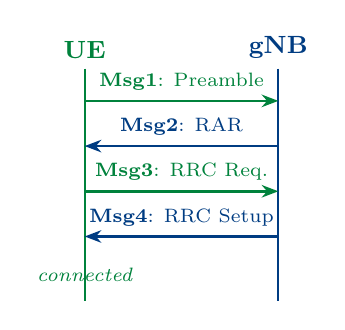
\begin{tikzpicture}[scale=0.82, every node/.style={font=\scriptsize}]
        % Lifelines
        \draw[thick, successgreen] (0,0) -- (0,-3.6);
        \draw[thick, ITUblue]      (3,0) -- (3,-3.6);

        % Labels
        \node[above, successgreen, font=\small\bfseries] at (0,0) {UE};
        \node[above, ITUblue,      font=\small\bfseries] at (3,0) {gNB};

        % Msg1
        \draw[arr=successgreen, line width=1pt] (0,-0.5) -- (3,-0.5)
              node[midway,above]{\textbf{Msg1}: Preamble};

        % Msg2
        \draw[arr=ITUblue, line width=1pt] (3,-1.2) -- (0,-1.2)
              node[midway,above]{\textbf{Msg2}: RAR};

        % Msg3
        \draw[arr=successgreen, line width=1pt] (0,-1.9) -- (3,-1.9)
              node[midway,above]{\textbf{Msg3}: RRC Req.};

        % Msg4
        \draw[arr=ITUblue, line width=1pt] (3,-2.6) -- (0,-2.6)
              node[midway,above]{\textbf{Msg4}: RRC Setup};

        % Connected label
        \node[successgreen, font=\scriptsize\itshape] at (0,-3.2) {connected};
        \draw[successgreen, dashed] (0,-2.8) -- (0,-3.1);
      \end{tikzpicture}
      \end{center}
    \end{column}
  \end{columns}

\end{frame}

% ── SLIDE: THE ATTACK ────────────────────────────────────────
\begin{frame}{The RRC Signaling Storm Attack}

  \begin{columns}[T]
    \begin{column}{0.52\textwidth}
      \textbf{Attack mechanism}

      \vspace{6pt}
      \begin{itemize}\setlength\itemsep{5pt}
        \item Adversary coordinates a botnet of compromised devices
        \item Each device sends RRC connection requests at high rate
        \item Combined rate: $\lambda_{\mathrm{high}} = 500\ \mathrm{req/s}$
              vs.\ normal $\lambda_{\mathrm{low}} = 10\ \mathrm{req/s}$
        \item RACH buffer saturates within seconds
        \item Access requests are dropped: \alert{QoS failure}
      \end{itemize}

      \vspace{8pt}
      Named \alert{\emph{RRC Signaling Storm}} in the literature \cite{b1}.
    \end{column}

    \begin{column}{0.46\textwidth}
      \begin{center}
      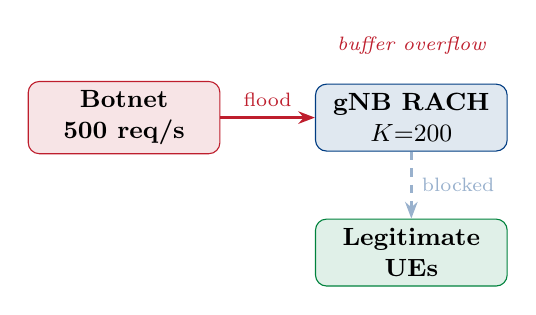
\begin{tikzpicture}[node distance=0.9cm and 1.2cm]
        \node[box=ITUred, text width=2.2cm] (bot)
              {Botnet\\500 req/s};
        \node[box=ITUblue, text width=2.2cm, right=1.2cm of bot] (gnb)
              {gNB RACH\\$K{=}200$};
        \node[box=successgreen, text width=2.2cm, below=0.85cm of gnb] (ue)
              {Legitimate UEs};

        \draw[arr=ITUred, line width=1.3pt]
              (bot) -- node[above,font=\scriptsize]{flood} (gnb);
        \draw[arr=ITUblue!40, dashed, line width=1pt]
              (gnb) -- node[right,font=\scriptsize]{blocked} (ue);
        \node[above=0.25cm of gnb, font=\scriptsize\itshape, text=ITUred]
              {buffer overflow};
      \end{tikzpicture}
      \end{center}

      \vspace{8pt}
      \begin{alertblock}{\small Impact}
        \small
        All connected services lose access until the attack subsides.
      \end{alertblock}
    \end{column}
  \end{columns}

\end{frame}

% ── SLIDE: CONTROL LOOP LATENCY ──────────────────────────────
\begin{frame}{Problem: Control Loop Latency in ACB/UAC}

  \textbf{Current defence:} Access Class Barring (ACB), 3GPP TS~38.331 UAC framework

  \vspace{10pt}
  \begin{center}
  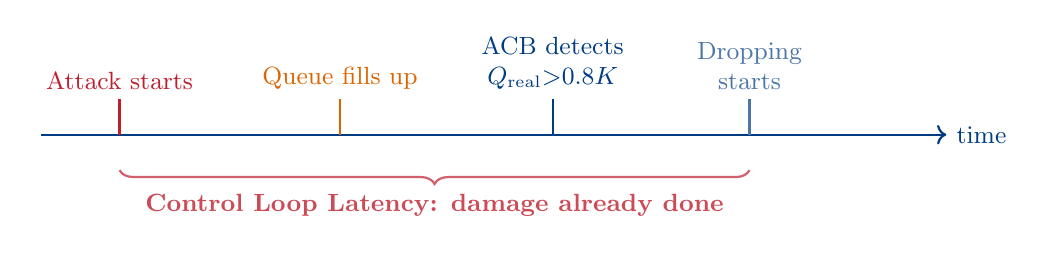
\begin{tikzpicture}[every node/.style={font=\small}]
    \draw[thick,->,ITUblue] (0,0) -- (11.5,0) node[right]{time};

    \foreach \x/\lbl/\col in {
        1/{Attack starts}/ITUred,
        3.8/{Queue fills up}/alertorange,
        6.5/{ACB detects $\qreal{>}0.8K$}/ITUblue,
        9/{Dropping starts}/ITUblue!70}{
      \draw[thick,\col] (\x,0) -- (\x,0.45);
      \node[above,\col,align=center,text width=2.1cm] at (\x,0.45){\lbl};
    }

    \draw[decorate,decoration={brace,amplitude=5pt,mirror},thick,ITUred!70]
      (1,-0.45) -- (9,-0.45)
      node[midway,below=5pt,ITUred!80,font=\small\bfseries]
           {Control Loop Latency: damage already done};
  \end{tikzpicture}
  \end{center}

  \vspace{6pt}
  \begin{columns}[T]
    \begin{column}{0.50\textwidth}
      \begin{alertblock}{\small Fundamental Causality Constraint}
        \small
        ACB throttles \textbf{only after} observing $\qreal > 0.8K$.
        During the build-up, requests are silently dropped.
      \end{alertblock}
    \end{column}
    \begin{column}{0.48\textwidth}
      \begin{block}{\small Empirical Evidence}
        \small
        Seo et al.\ (2021): random access delay requirements can be violated
        near unstable or saturated access regimes \cite{b6}.
      \end{block}
    \end{column}
  \end{columns}

\end{frame}

% ── SLIDE: RESEARCH GAP ──────────────────────────────────────
\begin{frame}{Research Gap: Existing Approaches}

  \begin{columns}[T]
    \begin{column}{0.32\textwidth}
      \begin{alertblock}{\small Reactive ACB / UAC}
        \small
        \textbf{Strength:} Simple, standards-compliant\\[4pt]
        \textbf{Limitation:} Reacts \textbf{after} saturation; inherent control loop latency
      \end{alertblock}
    \end{column}

    \begin{column}{0.32\textwidth}
      \begin{alertblock}{\small ML / DNN Predictors}
        \small
        \textbf{Strength:} High accuracy on stationary traffic\\[4pt]
        \textbf{Limitation:} $O(W)$ inference cost ($W\!\sim\!10^5$--$10^7$); millisecond latency, impractical on gNB hardware
      \end{alertblock}
    \end{column}

    \begin{column}{0.32\textwidth}
      \begin{alertblock}{\small Standard Digital Twin}
        \small
        \textbf{Strength:} Proactive control possible\\[4pt]
        \textbf{Limitation:} \alert{Model drift} under non-stationary traffic; state mirroring error grows unbounded
      \end{alertblock}
    \end{column}
  \end{columns}

  \vspace{10pt}
  \begin{exampleblock}{\small Research Gap}
    No existing DT approach suppresses model drift with an \textbf{online calibration loop}
    during the attack interval. This work closes that gap.
  \end{exampleblock}

\end{frame}

% =============================================================
\section{System Model}
% =============================================================

% ── SLIDE: SYSTEM MODEL ──────────────────────────────────────
\begin{frame}{System Model: MMPP/M/c/K Queue}

  \begin{columns}[T]
    \begin{column}{0.54\textwidth}
      \textbf{Two-state CTMC (Markov Modulated Poisson Process)}

      \vspace{4pt}
      Generator matrix:
      \[
        Q = \begin{bmatrix}
          -\alpha_{\mathrm{mmpp}} & \alpha_{\mathrm{mmpp}} \\
          \beta_{\mathrm{mmpp}}   & -\beta_{\mathrm{mmpp}}
        \end{bmatrix}
      \]

      \begin{itemize}\setlength\itemsep{3pt}
        \item $S_0$ (normal): $\lambda_{\mathrm{low}} = 10\ \mathrm{req/s}$
        \item $S_1$ (burst): $\lambda_{\mathrm{high}} = 500\ \mathrm{req/s}$
        \item $\alpha_{\mathrm{mmpp}} = 0.1\ \mathrm{s}^{-1}$,\;
              $\beta_{\mathrm{mmpp}} = 0.5\ \mathrm{s}^{-1}$
        \item Sojourn time $\sim \mathrm{Exp}(|Q_{ii}|)$
        {\footnotesize -- exact CTMC dynamics in DES, no matrix exponential needed}
      \end{itemize}
    \end{column}

    \begin{column}{0.44\textwidth}
      \begin{center}
      \vspace{6pt}
      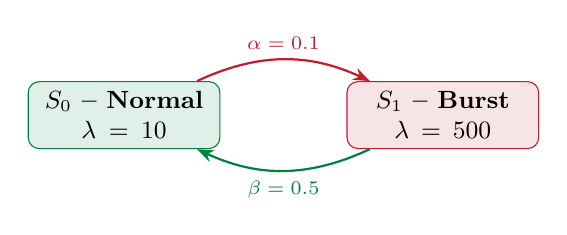
\begin{tikzpicture}
        \node[box=successgreen, text width=2.2cm] (s0)
              {$S_0$ -- Normal\\$\lambda=10$};
        \node[box=ITUred, text width=2.2cm, right=1.6cm of s0] (s1)
              {$S_1$ -- Burst\\$\lambda=500$};
        \draw[arr=ITUred, bend left=25]
              (s0) to node[above,font=\scriptsize]{$\alpha=0.1$} (s1);
        \draw[arr=successgreen, bend left=25]
              (s1) to node[below,font=\scriptsize]{$\beta=0.5$} (s0);
      \end{tikzpicture}
      \end{center}

      \vspace{8pt}
      \begin{block}{\small Physical gNB RACH}
        \small
        \renewcommand{\arraystretch}{1.2}
        \begin{tabular}{ll}
          Preamble channels & $c = 54$ \\
          Buffer capacity   & $K = 200$ \\
          Service time      & $\mathrm{Exp}(1)$ \\
        \end{tabular}
      \end{block}
    \end{column}
  \end{columns}

\end{frame}

% =============================================================
\section{Proposed Method}
% =============================================================

% ── SLIDE: METHOD OVERVIEW ───────────────────────────────────
\begin{frame}{Proposed Method: Calibrated Digital Twin}

  \begin{center}
  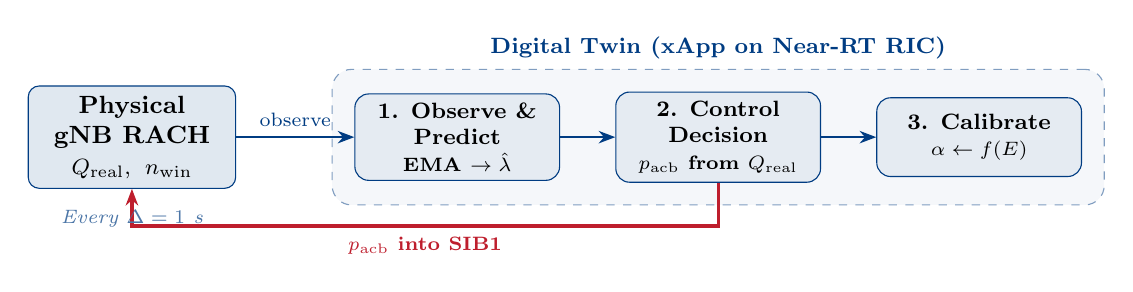
\begin{tikzpicture}[node distance=0.45cm and 0.9cm]

    % gNB
    \node[box=ITUblue, text width=2.4cm, minimum height=1.3cm] (gnb)
          {Physical\\gNB RACH\\{\footnotesize $\qreal,\;n_{\mathrm{win}}$}};

    % Three stages in a row to the right
    \node[stage, right=1.5cm of gnb] (obs)
          {1. Observe \&\\Predict\\{\scriptsize EMA $\to\hat\lambda$}};
    \node[stage, right=0.7cm of obs] (ctrl)
          {2. Control\\Decision\\{\scriptsize $\pacb$ from $\qreal$}};
    \node[stage, right=0.7cm of ctrl] (cal)
          {3. Calibrate\\{\scriptsize $\alpha \leftarrow f(E)$}};

    % DT bounding box
    \begin{scope}[on background layer]
      \node[rectangle, rounded corners=7pt, draw=ITUblue!50, fill=ITUblue!4, dashed,
            fit=(obs)(ctrl)(cal), inner sep=8pt,
            label={[font=\footnotesize\bfseries,ITUblue]above:Digital Twin (xApp on Near-RT RIC)}] {};
    \end{scope}

    % Pipeline arrows
    \draw[arr=ITUblue] (obs) -- (ctrl);
    \draw[arr=ITUblue] (ctrl) -- (cal);

    % gNB -> DT (observation)
    \draw[arr=ITUblue] (gnb.east) -- node[above,font=\scriptsize]{observe} (obs.west);

    % DT -> gNB (control), routed below
    \draw[arr=ITUred, line width=1.2pt]
          (ctrl.south) -- ++(0,-0.55) -| (gnb.south)
          node[pos=0.25, below, font=\scriptsize\bfseries, ITUred]{$\pacb$ into SIB1};

    \node[below=0.15cm of gnb, font=\scriptsize\itshape, text=ITUblue!70]
          {Every $\Delta=1$ s};
  \end{tikzpicture}
  \end{center}

  \vspace{6pt}
  \begin{columns}[c]
    \begin{column}{0.32\textwidth}\centering
      \footnotesize\textbf{Step 1}\\Count arrivals in window\\$\Rightarrow$ EMA predicts $\hat\lambda$
    \end{column}
    \begin{column}{0.33\textwidth}\centering
      \footnotesize\textbf{Step 2}\\Compute minimum barring probability\\to keep $\qreal < K$
    \end{column}
    \begin{column}{0.32\textwidth}\centering
      \footnotesize\textbf{Step 3}\\Adjust $\alpha$ via asymmetric\\step rule if $E > \varepsilon$
    \end{column}
  \end{columns}

\end{frame}

% ── SLIDE: EMA + p_acb ───────────────────────────────────────
\begin{frame}{EMA Predictor and ACB Control Policy}

  \begin{columns}[T]
    \begin{column}{0.48\textwidth}
      \textbf{EMA arrival rate predictor}
      \[
        \ema_t = \alpha \cdot \lambda_{\mathrm{cur}}
               + (1-\alpha) \cdot \ema_{t-1}
      \]
      {\small $\lambda_{\mathrm{cur}} = n_{\mathrm{win}} / \Delta$}

      \vspace{6pt}
      {\small
      \begin{itemize}\setlength\itemsep{3pt}
        \item Initial weight $\alpha_0 = 0.2$ (empirical default; stable before calibration)
        \item $\alpha$ is \textbf{dynamic}, updated by the calibration loop
      \end{itemize}}
    \end{column}

    \begin{column}{0.50\textwidth}
      \textbf{Stochastic barring probability}
      \[
        \pacb = \max\!\Bigl(0,\;\min\!\Bigl(1,\;
          1 - \tfrac{K - \qreal}{\max(\ema_t\cdot\Delta,\,10^{-9})}
        \Bigr)\Bigr)
      \]

      \vspace{4pt}
      {\small
      \begin{itemize}\setlength\itemsep{3pt}
        \item Minimum probability to prevent $\qreal \geq K$ next step
        \item Applied as Bernoulli trial per request
        \item Maps to \texttt{uac-BarringInfo} in SIB1, 3GPP TS~38.331 UAC
      \end{itemize}}
    \end{column}
  \end{columns}

  \vspace{8pt}
  \begin{exampleblock}{\small Key Insight}
    \small
    $\pacb$ rises \textbf{before} $\qreal$ reaches $K$: proactive throttling, not reactive.
  \end{exampleblock}

\end{frame}

% ── SLIDE: CALIBRATION LOOP ──────────────────────────────────
\begin{frame}{Continuous Calibration Loop}

  \begin{columns}[T]
    \begin{column}{0.52\textwidth}
      \textbf{State Mirroring Error}
      \[
        E(t) = \bigl|\qreal(t) - \qvirt(t)\bigr|
      \]

      \vspace{6pt}
      \textbf{Asymmetric step rule}
      \[
        \alpha \leftarrow \begin{cases}
          \min(\alpha_{\max},\;\alpha + \delta^{+}) & E > \varepsilon \\
          \max(\alpha_{\min},\;\alpha - \delta^{-}) & \text{otherwise}
        \end{cases}
      \]

      \vspace{4pt}
      {\small Parameters: $\varepsilon = 10$,\;
                  $\delta^{+} = 0.05$,\;
                  $\delta^{-} = 0.01$}
    \end{column}

    \begin{column}{0.46\textwidth}
      \textbf{Why asymmetric?}

      \vspace{6pt}
      \begin{block}{\small Attack onset: $\delta^{+} = 0.05$}
        \small
        Fast increase: EMA becomes high-frequency.
        Outdated observations discarded quickly.
      \end{block}

      \vspace{6pt}
      \begin{exampleblock}{\small Normal traffic: $\delta^{-} = 0.01$}
        \small
        Slow decay: statistical stability preserved.
        Avoids oscillation around $\varepsilon$.
      \end{exampleblock}

      \vspace{6pt}
      {\small $\delta^{+} \gg \delta^{-}$: rate mismatch is intentional.}
    \end{column}
  \end{columns}

\end{frame}

% ── SLIDE: ALGORITHM ─────────────────────────────────────────
\begin{frame}{Algorithm~1: Calibrated DT Control Loop}

  \begin{columns}[T]
    \begin{column}{0.60\textwidth}
      \setlength{\fboxsep}{5pt}
      \colorbox{lightgray}{%
      \begin{minipage}{0.96\linewidth}
        \footnotesize
        \textbf{Input:} $\qreal$,\; $n_{\mathrm{win}}$,\; $\Delta$,\;
                        $\varepsilon$,\; $\alpha$,\; $\alpha_{\min}$,\;
                        $\alpha_{\max}$,\; $\delta^{+}$,\; $\delta^{-}$\\[1pt]
        \textbf{Output:} $\pacb$,\; updated $\qvirt$,\; updated $\alpha$\\[3pt]
        \textbf{Every} $\Delta$ step:\\[1pt]
        \quad 1:\; $\lambda_{\mathrm{cur}} \leftarrow n_{\mathrm{win}} / \Delta$\\
        \quad 2:\; $\ema_t \leftarrow \alpha\cdot\lambda_{\mathrm{cur}}
                              + (1-\alpha)\cdot\ema_{t-1}$\\
        \quad 3:\; $d \leftarrow \max(\ema_t\cdot\Delta,\;10^{-9})$\\
        \quad 4:\; $\pacb \leftarrow \max(0,\min(1,\,1-(K-\qreal)/d))$\\
        \quad 5:\; $\qvirt \leftarrow \mathrm{clip}(\qvirt +
                              \ema_t(1{-}\pacb)\Delta - c\Delta,\;0,K)$\\
        \quad 6:\; $E \leftarrow |\qreal - \qvirt|$\\
        \quad 7:\; \textbf{if} $E > \varepsilon$:\;
                   $\alpha \leftarrow \min(\alpha_{\max},\,\alpha+\delta^{+})$\\
        \quad 8:\; \textbf{else}:\;
                   $\alpha \leftarrow \max(\alpha_{\min},\,\alpha-\delta^{-})$\\
        \quad 9:\; \texttt{drop\_rate} $\leftarrow \pacb$
      \end{minipage}}
    \end{column}

    \begin{column}{0.38\textwidth}
      \vspace{4pt}
      \begin{block}{\small O(1) per control step}
        \small
        \begin{itemize}\setlength\itemsep{3pt}
          \item Fixed arithmetic operations
          \item 4 state variables: $\{\ema_t,\;\qvirt,\;\alpha,\;n_{\mathrm{win}}\}$
          \item \textbf{O(1) time, O(1) space}
        \end{itemize}
      \end{block}

      \vspace{8pt}
      \begin{alertblock}{\small vs.\ DNN predictors}
        \small
        $O(W)$, $W\!\sim\!10^5$--$10^7$\\
        Latency: milliseconds\\
        gNB requires: \textbf{microseconds}
      \end{alertblock}
    \end{column}
  \end{columns}

\end{frame}

% =============================================================
\section{Results \& Evaluation}
% =============================================================

% ── SLIDE: SIMULATION SETUP ──────────────────────────────────
\begin{frame}{Simulation Setup}

  \begin{columns}[T]
    \begin{column}{0.46\textwidth}
      \textbf{Experimental configuration}

      \vspace{4pt}
      \begin{itemize}\setlength\itemsep{3pt}
        \item Discrete-event simulation: SimPy, Python 3.10
        \item $T_{\mathrm{sim}} = 1000\ \mathrm{s}$ per run
        \item $N = 10$ independent seeds (Monte Carlo)
        \item 95\% CI: $\bar{x} \pm 1.96\,\hat\sigma/\sqrt{N}$
      \end{itemize}
    \end{column}

    \begin{column}{0.52\textwidth}
      \textbf{Key parameters}

      \vspace{4pt}
      \renewcommand{\arraystretch}{1.15}
      \begin{tabular}{lll}
        \toprule
        Parameter & Symbol & Value \\
        \midrule
        Preamble channels & $c$ & 54 \\
        Buffer capacity & $K$ & 200 \\
        Normal arrival rate & $\lambda_{\mathrm{low}}$ & 10 req/s \\
        Burst arrival rate & $\lambda_{\mathrm{high}}$ & 500 req/s \\
        Control interval & $\Delta$ & 1 s \\
        Calibration threshold & $\varepsilon$ & 10 \\
        Initial EMA weight & $\alpha_0$ & 0.20 \\
        \bottomrule
      \end{tabular}
    \end{column}
  \end{columns}

  \vspace{6pt}
  \textbf{Three methods compared:}\quad
  \textcolor{alertorange}{\textbf{Reactive Baseline}} (threshold $0.8K$, drop 0.5)\quad
  \textcolor{ITUblue!70}{\textbf{DT no-calib.}} ($\alpha$ fixed)\quad
  \textcolor{ITUblue}{\textbf{Calibrated DT}} (asymmetric step rule)

\end{frame}

% ── SLIDE: STATE MIRRORING ERROR ─────────────────────────────
\begin{frame}{Result 1: State Mirroring Error -- 42\% Reduction}

  \begin{center}
    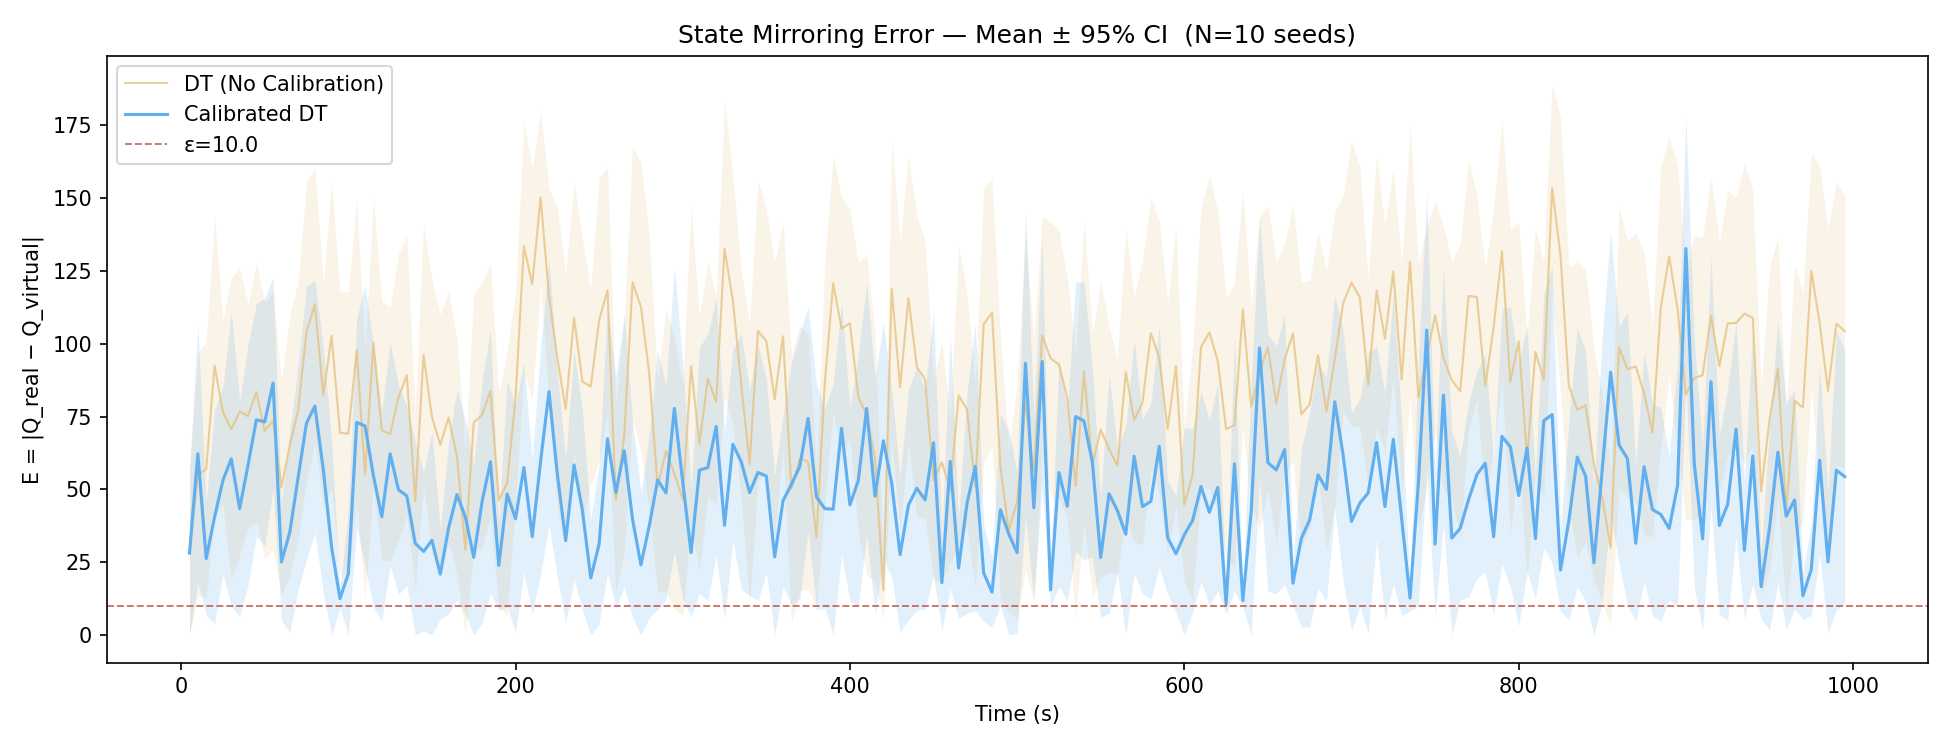
\includegraphics[height=3.8cm]{phase5_E_ci.png}
  \end{center}

  \begin{columns}[T]
    \begin{column}{0.48\textwidth}
      \begin{block}{\small $E_{\mathrm{mean}}$ ($N=10$, 95\% CI)}
        \footnotesize
        \renewcommand{\arraystretch}{1.2}
        \begin{tabular}{lc}
          \toprule
          Method & $E_{\mathrm{mean}}$ \\
          \midrule
          DT (no calib.) & $85.03 \pm 4.40$ \\
          \textbf{Calib.\ DT} & $\mathbf{49.14 \pm 3.09}$ \\
          \bottomrule
        \end{tabular}
      \end{block}
    \end{column}

    \begin{column}{0.50\textwidth}
      \begin{alertblock}{\small Key Result}
        \footnotesize
        $(85.03 - 49.14) / 85.03 \approx \mathbf{42\%}$ reduction.\\[3pt]
        Calibration suppresses model drift continuously during burst.
      \end{alertblock}
    \end{column}
  \end{columns}

\end{frame}

% ── SLIDE: QUEUE STABILITY ───────────────────────────────────
\begin{frame}{Result 2: Queue Stability}

  \begin{center}
    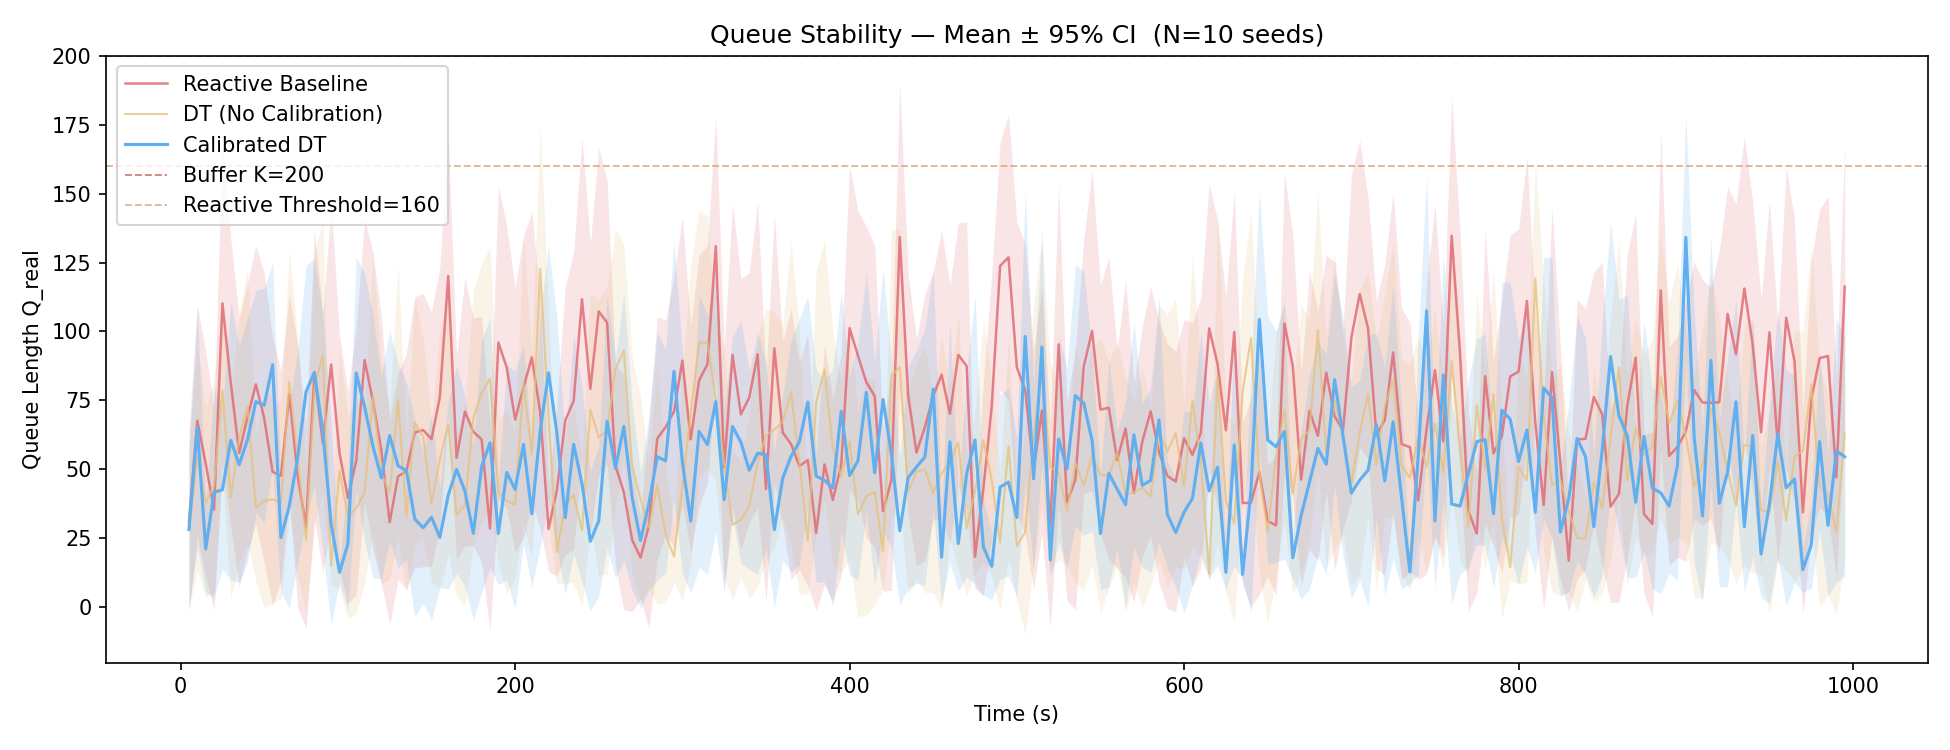
\includegraphics[height=3.3cm]{phase5_q_real_ci.png}
  \end{center}

  \begin{columns}[T]
    \begin{column}{0.48\textwidth}
      \begin{block}{\small $P_{success}$ ($N=10$, 95\% CI)}
        \footnotesize
        \renewcommand{\arraystretch}{1.1}
        \begin{tabular}{lc}
          \toprule
          Method & $P_{success}$ \\
          \midrule
          Reactive & $0.310 \pm 0.015$ \\
          DT (no calib.) & $0.301 \pm 0.011$ \\
          \textbf{Calib.\ DT} & $\mathbf{0.309 \pm 0.019}$ \\
          \bottomrule
        \end{tabular}
      \end{block}
    \end{column}

    \begin{column}{0.50\textwidth}
      \begin{exampleblock}{\small Interpretation}
        \footnotesize
        Reactive reacts only after $\qreal > 0.8K$.\\[2pt]
        Calibrated DT raises $\pacb$ \textbf{before} saturation: queue stays in stable region.
      \end{exampleblock}
    \end{column}
  \end{columns}

\end{frame}

% ── SLIDE: DELAY CDF ─────────────────────────────────────────
\begin{frame}{Result 3: Queueing Delay CDF}

  \begin{center}
    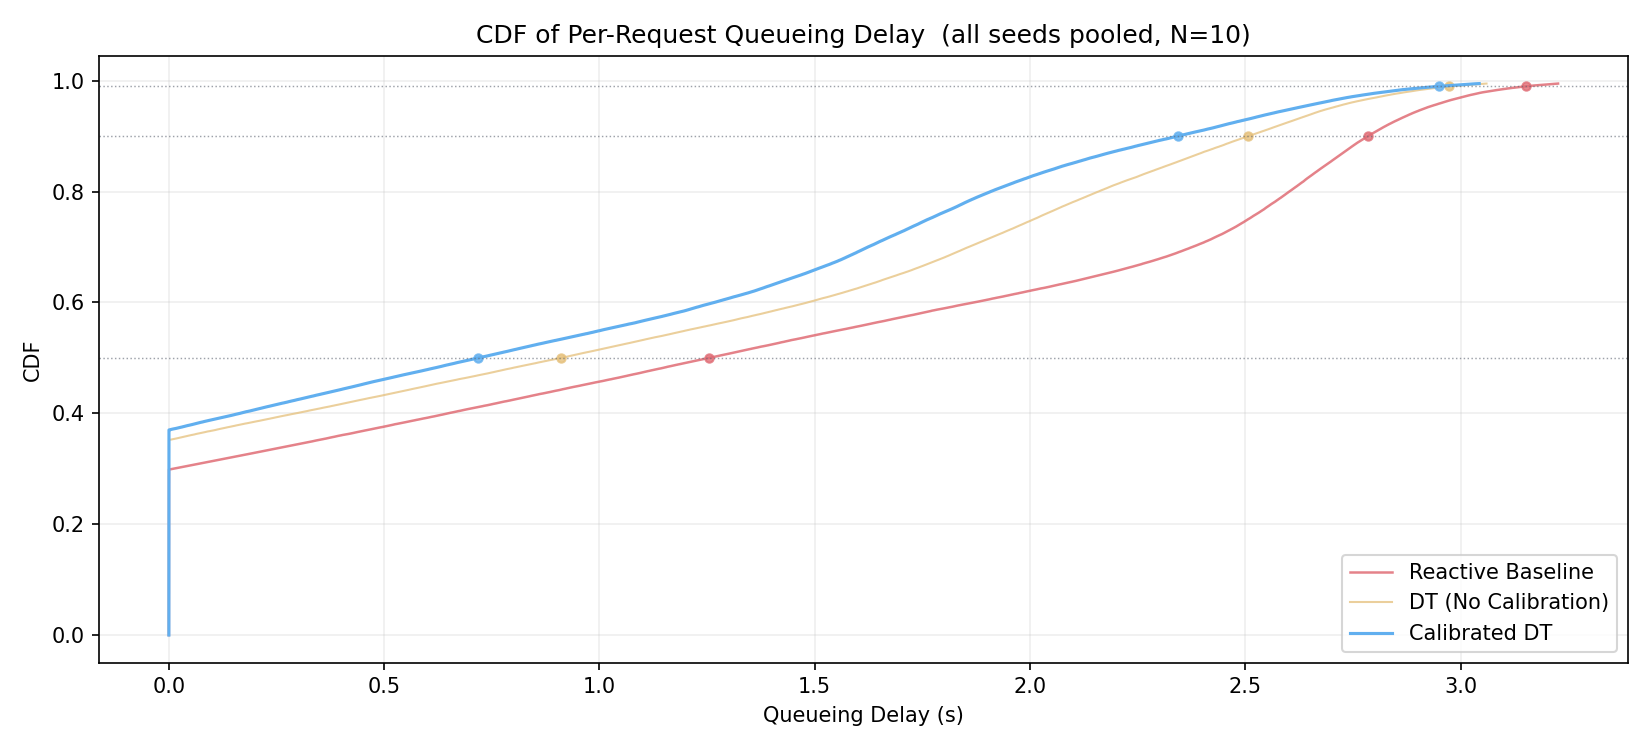
\includegraphics[height=3.8cm]{phase5_delay_cdf.png}
  \end{center}

  \begin{columns}[T]
    \begin{column}{0.48\textwidth}
      \begin{block}{\small CDF Left-Shift}
        \footnotesize
        Calibrated DT curve is shifted left: lower delay at the reported percentiles.
      \end{block}
    \end{column}

    \begin{column}{0.50\textwidth}
      \begin{exampleblock}{\small Why tail is suppressed}
        \footnotesize
        Reactive allows queuing near saturation: large P90/P99 spikes.\\[3pt]
        Calibrated DT holds $\qreal$ in stable region: equivalent success rate with lower served-request delay.
      \end{exampleblock}
    \end{column}
  \end{columns}

\end{frame}

% ── SLIDE: EPSILON SENSITIVITY ───────────────────────────────
\begin{frame}{Result 4: $\varepsilon$ Sensitivity Analysis}

  \begin{center}
    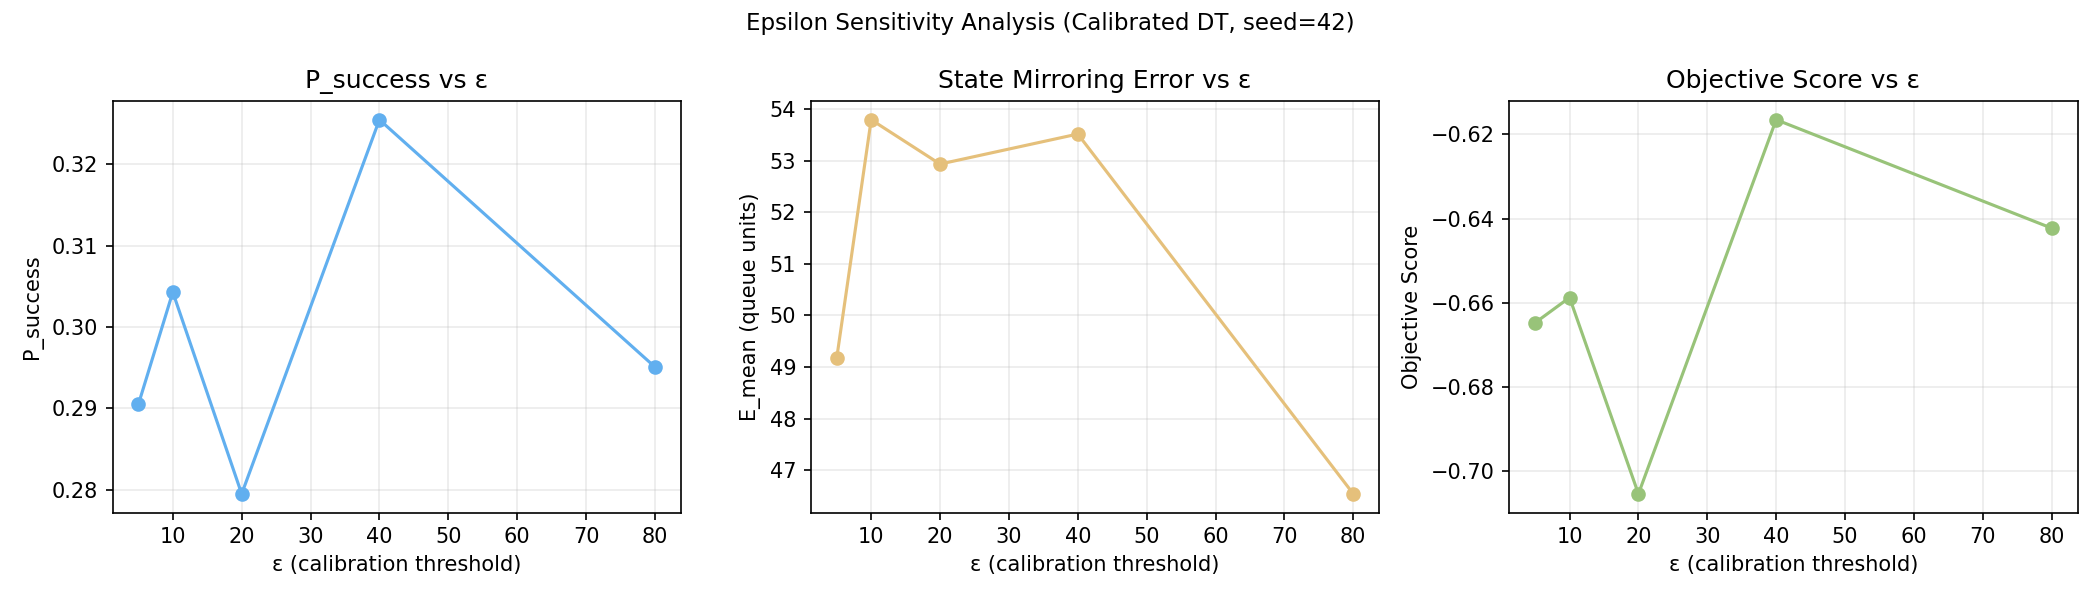
\includegraphics[height=3.8cm]{phase5_epsilon_sensitivity.png}
  \end{center}

  \begin{columns}[T]
    \begin{column}{0.48\textwidth}
      \begin{block}{\small Tested: $\varepsilon \in \{5,\;10,\;20,\;40,\;80\}$}
        \footnotesize
        Single-seed sweep (seed=42): $\varepsilon=40$ achieves highest composite objective; $\varepsilon=10$ adopted as conservative default just above normal-traffic noise floor.
      \end{block}
    \end{column}

    \begin{column}{0.50\textwidth}
      \begin{exampleblock}{\small Interpretation}
        \footnotesize
        \textbf{Too small} ($\varepsilon=5$): over-calibrates in normal traffic.\\[3pt]
        \textbf{Too large} ($\varepsilon=80$): calibration rarely triggers.\\[3pt]
        Multi-seed validation needed; $\varepsilon=10$ used as conservative default.
      \end{exampleblock}
    \end{column}
  \end{columns}

\end{frame}

% ── SLIDE: O-RAN DEPLOYMENT ──────────────────────────────────
\begin{frame}{O(1) Complexity and O-RAN Deployment}

  \begin{columns}[T]
    \begin{column}{0.50\textwidth}
      \textbf{Complexity comparison}

      \vspace{4pt}
      \begin{block}{\small Calibrated DT: O(1) per step}
        \small
        \begin{itemize}\setlength\itemsep{3pt}
          \item Fixed arithmetic, 4 state variables
          \item Fixed-cost arithmetic per control step
          \item Suitable for tight gNB control budgets after hardware benchmarking
        \end{itemize}
      \end{block}

      \vspace{6pt}
      \begin{alertblock}{\small DNN predictors: O(W)}
        \small
        $W\!\sim\!10^5$--$10^7$ weights.
        Inference latency: milliseconds.
        \textbf{Impractical on gNB hardware.}
      \end{alertblock}
    \end{column}

    \begin{column}{0.48\textwidth}
      \textbf{O-RAN integration}

      \vspace{4pt}
      \begin{center}
      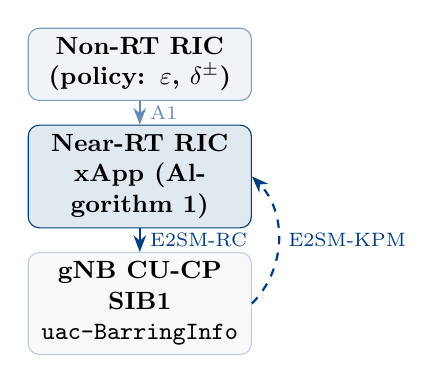
\begin{tikzpicture}[node distance=0.3cm, every node/.style={font=\scriptsize}]
        \node[box=ITUblueMid, text width=2.6cm] (nonrt)
              {Non-RT RIC\\(policy: $\varepsilon$, $\delta^\pm$)};
        \node[box=ITUblue, text width=2.6cm, below=0.3cm of nonrt] (nearrt)
              {Near-RT RIC\\xApp (Algorithm 1)};
        \node[box=ITUblueLight, text width=2.6cm, below=0.3cm of nearrt] (gnb)
              {gNB CU-CP\\SIB1 \texttt{uac-BarringInfo}};

        \draw[arr=ITUblue!60] (nonrt) -- node[right]{A1} (nearrt);
        \draw[arr=ITUblue] (nearrt) -- node[right]{E2SM-RC} (gnb);
        \draw[arr=ITUblue, dashed, bend right=45]
              (gnb.east) to node[right]{E2SM-KPM} (nearrt.east);
      \end{tikzpicture}
      \end{center}

      \vspace{2pt}
      {\scriptsize
      \begin{itemize}\setlength\itemsep{1pt}
        \item $\Delta=1$ s fits Near-RT RIC range (10 ms to 1 s)
        \item No protocol modifications required
        \item Vendor-independent xApp
      \end{itemize}}
    \end{column}
  \end{columns}

\end{frame}

% =============================================================
\section{Conclusion}
% =============================================================

% ── SLIDE: CONCLUSION ────────────────────────────────────────
\begin{frame}{Conclusion and Future Work}

  \begin{columns}[T]
    \begin{column}{0.50\textwidth}
      \textbf{Three key results}

      \vspace{6pt}
      \begin{enumerate}\setlength\itemsep{6pt}
        \item \textbf{42\% reduction} in state mirroring error\\
              (calibrated vs.\ uncalibrated DT)

        \item $P_{success}$ \textbf{statistically equivalent} to reactive baseline;
              P90/P99 queueing delay \textbf{reduced}

        \item \textbf{O(1) complexity}: deployable within commercial gNB software via O-RAN xApp
      \end{enumerate}

      \vspace{8pt}
      \begin{exampleblock}{\small Central Finding}
        \small
        Proactive control in non-stationary 5G environments requires both a
        sound control policy \textbf{and} tight virtual-physical alignment.
      \end{exampleblock}
    \end{column}

    \begin{column}{0.48\textwidth}
      \textbf{Future work}

      \vspace{6pt}
      \begin{itemize}\setlength\itemsep{8pt}
        \item \textbf{Multi-cell extension:} current model treats one gNB cell independently.
              Real deployments involve handover correlations and inter-cell interference.
              Requires a distributed DT architecture with inter-cell state sharing.

        \item \textbf{RL-based calibration:} fixed $\delta^{+}$, $\delta^{-}$ are vulnerable to
              slow ramp-up attacks. An RL agent can learn these step sizes dynamically using
              state mirroring error as a reward signal.
      \end{itemize}
    \end{column}
  \end{columns}

\end{frame}

% ── Q&A ──────────────────────────────────────────────────────
{
\setbeamertemplate{footline}{}
\begin{frame}[noframenumbering,c]
  \begin{center}
    {\LARGE\bfseries\color{ITUblue} Questions?}

    \vspace{20pt}
    {\large 5G RRC Signaling Storm Mitigation\\
    via a Proactive Digital Twin Architecture with Continuous Calibration}

    \vspace{16pt}
    \begin{tabular}{ll}
      \textbf{Author:}  & Omer Dikyol \\
      \textbf{Email:}   & dikyol25@itu.edu.tr \\
      \textbf{Course:}  & BLG 632E, ITU \\
    \end{tabular}
  \end{center}
\end{frame}
}

% ── REFERENCES ───────────────────────────────────────────────
\begin{frame}[allowframebreaks]{References}
  \footnotesize
  \begin{thebibliography}{9}

  \bibitem{b1}
  A. Tabiban et al.,
  ``Signaling Storm in O-RAN,''
  \emph{IEEE Commun. Mag.}, vol.~62, no.~6, Jun.~2024.

  \bibitem{b2}
  B. H. Lee et al.,
  ``Enhanced Random Access for Massive-MTC,''
  \emph{IEEE Internet of Things J.}, vol.~8, no.~8, pp.~7046--7064, Apr.~2021.

  \bibitem{b3}
  M. Grieves and J. Vickers,
  ``Digital Twin: Mitigating Unpredictable Emergent Behavior,''
  Springer, 2017.

  \bibitem{b4}
  3GPP, ``NR; RRC Protocol Specification,'' TS~38.331, version~17.3.0, Release~17, Jan.~2023.

  \bibitem{b5}
  L. Miuccio et al.,
  ``Joint Control of Random Access for Massive MTC in 5G NR,''
  \emph{IEEE Internet of Things J.}, vol.~7, no.~6, Jun.~2020.

  \bibitem{b6}
  J.-B. Seo et al.,
  ``Analysis of Two-Step Random Access Procedure for Cellular URLLC,''
  \emph{IEEE Access}, vol.~9, Jan.~2021.

  \bibitem{b7}
  S. K. Sharma and X. Wang,
  ``Toward Massive MTC in Ultra-Dense Cellular IoT Networks,''
  \emph{IEEE Commun. Surveys Tuts.}, vol.~22, no.~1, 2020.

  \bibitem{b8}
  R. Dong et al.,
  ``Deep Learning for Radio Resource Allocation in 5G,''
  \emph{IEEE Trans. Wireless Commun.}, vol.~20, no.~4, Apr.~2021.

  \bibitem{b9}
  C. Zhang et al.,
  ``Deep Learning in Mobile and Wireless Networking: A Survey,''
  \emph{IEEE Commun. Surveys Tuts.}, vol.~21, no.~3, 2019.

  \bibitem{b10}
  H. X. Nguyen et al.,
  ``Digital Twin for 5G and Beyond,''
  \emph{IEEE Commun. Mag.}, vol.~59, no.~2, Feb.~2021.

  \bibitem{b11}
  P. Almasan et al.,
  ``Network Digital Twin: Context, Enabling Technologies, and Opportunities,''
  \emph{IEEE Commun. Mag.}, vol.~60, no.~11, Nov.~2022.

  \bibitem{b12}
  R. F. Olimid and G. Nencioni,
  ``5G Network Slicing: A Security Overview,''
  \emph{IEEE Access}, vol.~8, Jun.~2020.

  \bibitem{b13}
  Q. Xu et al.,
  ``Digital Twin-Based Anomaly Detection in Cyber-Physical Systems,''
  \emph{Proc. IEEE ICST}, Apr.~2021.

  \bibitem{b14}
  M. Polese et al.,
  ``Understanding O-RAN,''
  \emph{IEEE Commun. Surveys Tuts.}, vol.~25, no.~2, 2023.

  \end{thebibliography}
\end{frame}

\end{document}
